% Created 2020-01-27 Mon 15:49
% Intended LaTeX compiler: pdflatex
\documentclass[11pt,letterpaper]{article}
\usepackage[utf8]{inputenc}
\usepackage[T1]{fontenc}
\usepackage{graphicx}
\usepackage{grffile}
\usepackage{longtable}
\usepackage{wrapfig}
\usepackage{rotating}
\usepackage[normalem]{ulem}
\usepackage{amsmath}
\usepackage{textcomp}
\usepackage{amssymb}
\usepackage{capt-of}
\usepackage{hyperref}
\usepackage[letterpaper,margin=1.3in]{geometry}
\usepackage{plex-mono}
\usepackage[sfdefault]{plex-sans}
\linespread{1.5} % Change line spacing
\usepackage{xcolor}
\usepackage{soul}
\usepackage{helvet}
\usepackage{listings}
\usepackage{inconsolata}
\usepackage{xcolor-solarized}
\definecolor{foreground}{RGB}{184, 83, 83} % For verbatim
\definecolor{background}{RGB}{255, 231, 231} % For verbatim
\let\OldTexttt\texttt
\renewcommand{\texttt}[1]{\OldTexttt{\footnotesize\colorbox{background}{\textcolor{foreground}{#1}}}}
\newenvironment{helvetica}{\fontfamily{phv}\selectfont}{\par}
\usepackage{hyperref} % Make the hyper-links prettier
\hypersetup{
colorlinks=true,
linkcolor=blue!70!white,
urlcolor=blue!95!black
}
\usepackage{enumitem}
\setlist[1]{itemsep=5pt}
\lstdefinelanguage{cpp}{
language=C++,
morekeywords={cerr,exit,string},
deletekeywords={...},
escapeinside={\%*}{*)},
showspaces=false,
showstringspaces=false,
showtabs=false,
stepnumber=1,
tabsize=4,
breakatwhitespace=false,
breaklines=true,
backgroundcolor=\color{solarized-base3},
basicstyle=\scriptsize\ttfamily\color{solarized-base0},
commentstyle=\itshape\color{solarized-base01},
keywordstyle=\color{solarized-green},
identifierstyle=\color{solarized-blue},
stringstyle=\color{solarized-cyan},
moredelim = *[l][\color{solarized-orange}]{\#},
moredelim = **[s][\color{solarized-cyan}]{<}{>},
rulecolor=\color{black},
literate={{\%d}}{{\textcolor{solarized-red}{\%d}}}2
{{\%2d}}{{\textcolor{solarized-red}{\%2d}}}3
{{\\n}}{{\textcolor{solarized-red}{\textbackslash{}n}}}2,
}
\author{Justin Kaipada - 100590167}
\date{\today}
\title{LAB 1 - REPORT}
\hypersetup{
 pdfauthor={Justin Kaipada - 100590167},
 pdftitle={LAB 1 - REPORT},
 pdfkeywords={},
 pdfsubject={},
 pdfcreator={Emacs 26.3 (Org mode 9.2.6)}, 
 pdflang={English}}
\begin{document}

\maketitle
\newpage % Go to the next page after title page

\section*{Task \#1: Encryption using different ciphers and modes}
\label{sec:orgd05415f}
\lstset{language=cpp,label= ,caption= ,captionpos=b,numbers=none}
\begin{lstlisting}
openssl enc -aes-128-cbc -e -in plain_text.txt -out cipher1.bin \
-K 000102030405060708090a0b0c0d0e0f \
-iv 000102030405060708090a0b0c0d0e0f

openssl enc -aes-128-cfb -e -in plain_text.txt -out cipher2.bin \
-K 000102030405060708090a0b0c0d0e0f \
-iv 000102030405060708090a0b0c0d0e0f

openssl enc -aes-192-gcm -e -in plain_text.txt -out cipher3.bin \
-K 000102030405060708090a0b0c0d0e0f \
-iv 000102030405060708090a0b0c0d0e0f

openssl enc -des-ede3-cfb1 -e -in plain_text.txt -out cipher4.bin \
-K 000102030405060708090a0b0c0d0e0f \
-iv 000102030405060708090a0b0c0d0e0f
\end{lstlisting}

In the above 4 commands used, the 3rd one failed saying \texttt{enc: AEAD ciphers not supported}. This was
a simple task that introduced us to the basics of using openssl to encrypt files.

\section*{Task \#2: Encryption Mode - ECB vs CBC}
\label{sec:org32699b5}

After encrypting the file using an ecb encryption algorithm and correcting the header information,
the image is somewhat representative of the original image, at least I can tell there is an outline
of the original image preserved in the encrypted file. The encrypted file can be viewed in
\texttt{pic\_ecb.bmp}.

After modifying the file header information the file produced as a result of the ecb encryption, it
didn't look anything like the original picture. The file \texttt{pic\_cbc.bmp} shoes the encrypted image
with corrected header and as you can see the whole image is disfigured.

\begin{center}
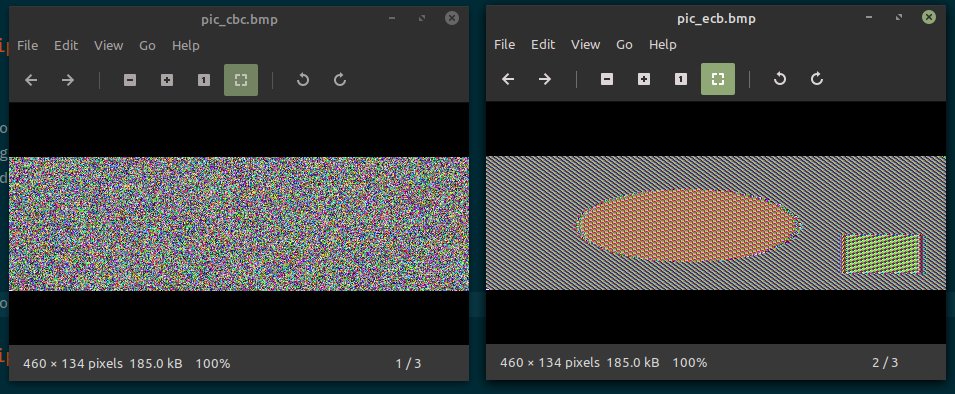
\includegraphics[width=.9\linewidth]{/home/justin/Desktop/Screenshot from 2020-01-27 10-58-20.png}
\end{center}

\section*{Task \#3: Encryption Mode - Corrupted Cipher Text}
\label{sec:org7d0dd8e}

Commands used for encryption
\lstset{language=sh,label= ,caption= ,captionpos=b,numbers=none}
\begin{lstlisting}
openssl enc -aes-128-ecb -e -in plain_text.txt -out task3ecb.bin \
-K 000102030405060708090a0b0c0d0e0f \
-iv 000102030405060708090a0b0c0d0e0f

openssl enc -aes-128-cbc -e -in plain_text.txt -out task3cbc.bin \
-K 000102030405060708090a0b0c0d0e0f \
-iv 000102030405060708090a0b0c0d0e0f

openssl enc -aes-128-cfb -e -in plain_text.txt -out task3cfb.bin \
-K 000102030405060708090a0b0c0d0e0f \
-iv 000102030405060708090a0b0c0d0e0f

openssl enc -aes-128-ofb -e -in plain_text.txt -out task3ofb.bin \
-K 000102030405060708090a0b0c0d0e0f \
-iv 000102030405060708090a0b0c0d0e0f
\end{lstlisting}

Before deciphering the files I say ecb will the be most affected by corruption and ofb will be least
affected, because ofb uses XOR operation on the bits so messing with one byte should only affect 1
byte when deciphering.

Commands used for decryption
\lstset{language=sh,label= ,caption= ,captionpos=b,numbers=none}
\begin{lstlisting}
openssl enc -aes-128-ecb -d -in task3ecb_c.bin -out plain_text_ecb.txt \
-K 000102030405060708090a0b0c0d0e0f \
-iv 000102030405060708090a0b0c0d0e0f

openssl enc -aes-128-cbc -d -in task3cbc_c.bin -out plain_text_cbc.txt \
-K 000102030405060708090a0b0c0d0e0f \
-iv 000102030405060708090a0b0c0d0e0f

openssl enc -aes-128-cfb -d -in task3cfb_c.bin -out plain_text_cfb.txt \
-K 000102030405060708090a0b0c0d0e0f \
-iv 000102030405060708090a0b0c0d0e0f

openssl enc -aes-128-ofb -d -in task3ofb_c.bin -out plain_text_ofb.txt \
-K 000102030405060708090a0b0c0d0e0f \
-iv 000102030405060708090a0b0c0d0e0f
\end{lstlisting}

After generating the encrypted file I corrupted them by replacing a random byte with a random
character using the hex editor. It seems like after deciphering the corrupted files the damage done
is more or less the same.

\textbf{CBC} This algorithm XOR’s a raw text against an IV then encrypts it and propagates that encrypted
cyphertext to be the next block’s IV. So if a byte if corrupted the data following that will most
likely get lost.
\begin{center}
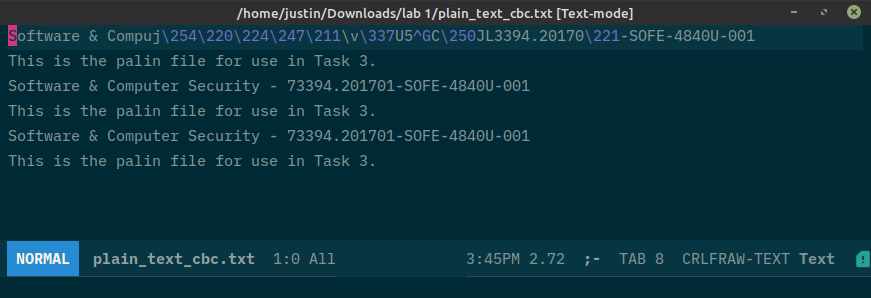
\includegraphics[width=.9\linewidth]{/home/justin/Desktop/cbc.png}
\end{center}

\textbf{ECB} This algorithm encrypts each block of plaintext to a corresponding ciphertext block, so if
byte is changed only that byte will get affected when deciphering back.
\begin{center}
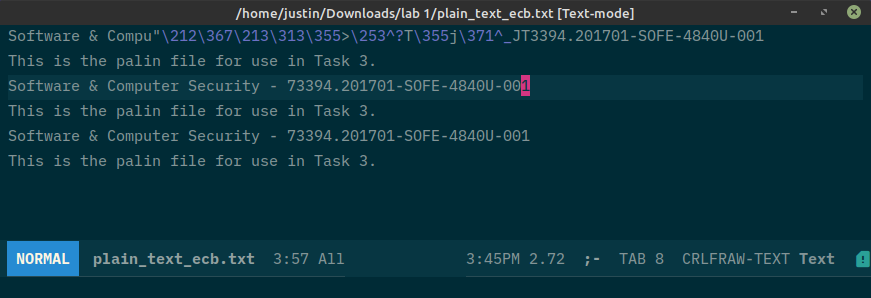
\includegraphics[width=.9\linewidth]{/home/justin/Desktop/ecb.png}
\end{center}

\textbf{CFB} This algorithm is like CBC but is also self-synchronizing. It is able to recover the data if
some of the encrypted text is lost or messed up. There may be a lot of data after the corrupted byte
affected, the algorithm will try to self correct.
\begin{center}
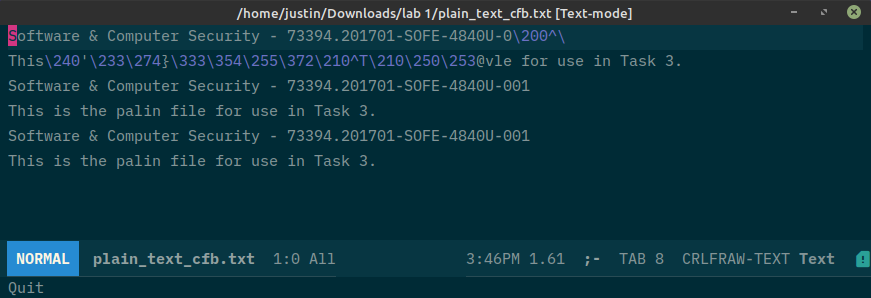
\includegraphics[width=.9\linewidth]{/home/justin/Desktop/cfb.png}
\end{center}

\textbf{OFB} This algorithm should be resistant to corruption of encrypted data. Only the bits that
are modified in error will be lost. Neighbouring bits should be unaffected.
\begin{center}
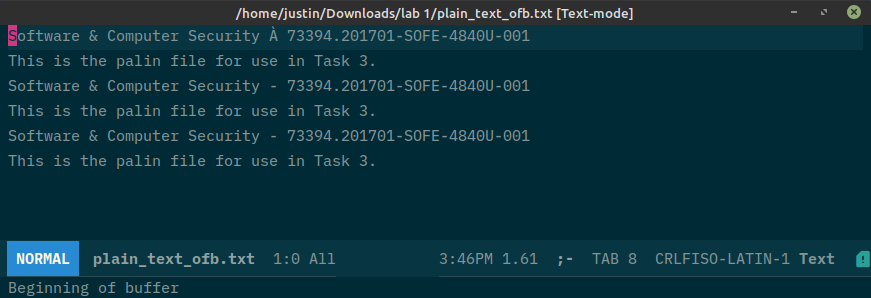
\includegraphics[width=.9\linewidth]{/home/justin/Desktop/ofb.png}
\end{center}

The implication is that different encryption methods must be chosen based on use cases and OFB seems
to be an algorithm which is least affected by corrupted bytes, because the neighbouring bits of the
corrupted bit is unaffected.
\section*{Task \#4: Pseudo random number generation}
\label{sec:orgc24cf46}

In this task we learned how to generate good random numbers, strong enough for security standards.

After running the command to see kernels entropy
\begin{center}
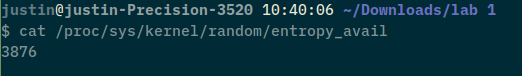
\includegraphics[width=.9\linewidth]{/home/justin/Desktop/Screenshot from 2020-01-27 11-44-41.png}
\end{center}

After moving the cursor and typing some stuff the entropy number seems to be changing every time
\begin{center}
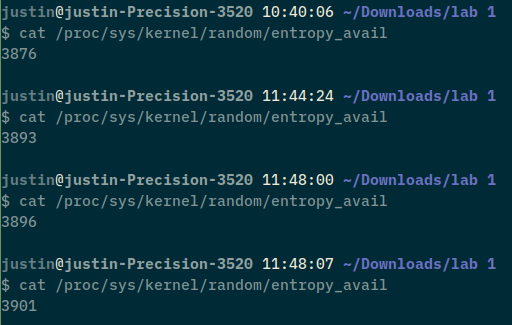
\includegraphics[width=.9\linewidth]{/home/justin/Desktop/Screenshot from 2020-01-27 11-49-56.png}
\end{center}

For next task we explore \texttt{/dev/random}. Running \texttt{head -c 16 /dev/random | hexdump} several times we
can see it generates 16 bytes of sudo random numbers very quickly.

\begin{center}
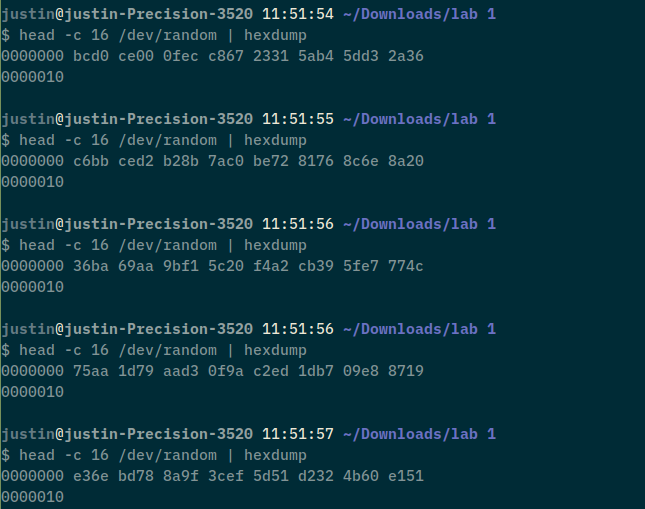
\includegraphics[width=.9\linewidth]{/home/justin/Desktop/Screenshot from 2020-01-27 11-52-16.png}
\end{center}

Once it gets blocked we can unblock it providing input to the system. Which is by moving the mouse
and typing anything into the keyboard.

Using \texttt{/dev/urandom} to generate unblocking pseudo random numbers 

\lstset{language=cpp,label= ,caption= ,captionpos=b,numbers=none}
\begin{lstlisting}
head -c 1600 /dev/urandom | hexdump
\end{lstlisting}

Ran this command a lot of times and it never blocked.
\end{document}